\documentclass[a4paper, 11pt, margin=1in]{article}
\usepackage[inline]{enumitem}
\usepackage{color}

\renewcommand{\baselinestretch}{1.15}

%%%%%%%%%%%%%%%%%%%%%%%%%%%%%%%%%%%%%%%%%%%%%Timeline%%%%%%%%%%%%
\usepackage[margin=3cm]{geometry}
\usepackage{ragged2e}
\usepackage{fourier}
\usepackage{tikz} 
\usetikzlibrary{chains,shapes.arrows,fit}

\definecolor{arrowcolor}{RGB}{201,216,232}% color for the arrow filling
\definecolor{circlecolor}{RGB}{79,129,189}% color for the inner circles filling
\colorlet{textcolor}{white}% color for the text inside the circles
\colorlet{bordercolor}{white}% color for the outer border of circles

\pgfdeclarelayer{background}
\pgfsetlayers{background,main}

\newcounter{task}

\newlength\taskwidth% width of the box for the task description
\newlength\taskvsep% vertical distance between the task description and arrow

\setlength\taskwidth{2.5cm}
\setlength\taskvsep{17pt}

\def\taskpos{}
\def\taskanchor{}

\newcommand\task[1]{%
  {\parbox[t]{\taskwidth}{\scriptsize\Centering#1}}}

\tikzset{
inner/.style={
  on chain,
  circle,
  inner sep=4pt,
  fill=circlecolor,
  line width=1.5pt,
  draw=bordercolor,
  text width=1.2em,
  align=center,
  text height=1.25ex,
  text depth=0ex
},
on grid
}

\newcommand\Task[2][]{%
\node[inner xsep=0pt] (c1) {\phantom{A}};
\stepcounter{task}
\ifodd\thetask\relax
  \renewcommand\taskpos{\taskvsep}\renewcommand\taskanchor{south}
\else
  \renewcommand\taskpos{-\taskvsep}\renewcommand\taskanchor{north}
\fi
\node[inner,font=\footnotesize\sffamily\color{textcolor}]    
  (c\the\numexpr\value{task}+1\relax) {#1};
\node[anchor=\taskanchor,yshift=\taskpos] 
  at (c\the\numexpr\value{task}+1\relax) {\task{#2}};
}

\newcommand\drawarrow{% the arrow is placed in the background layer 
                                                     % after the node for the tasks have been placed
\ifnum\thetask=0\relax
  \node[on chain] (c1) {}; % if no \Task command is used, the arrow will be drawn
\fi
\node[on chain] (f) {};
\begin{pgfonlayer}{background}
\node[
  inner sep=10pt,
  single arrow,
  single arrow head extend=0.8cm,
  draw=none,
  fill=arrowcolor,
  fit= (c1) (f)
] (arrow) {};
\fill[white] % the decoration at the tail of the arrow
  (arrow.before tail) -- (c1|-arrow.west) -- (arrow.after tail) -- cycle;
\end{pgfonlayer}
}

\newenvironment{timeline}[1][node distance=.75\taskwidth]
  {\par\noindent\begin{tikzpicture}[start chain,#1]}
  {\drawarrow\end{tikzpicture}\par}
%%%%%%%%%%%%%%%%%%%%%%%%%%%%%%%%%%%%%%%%%%%%%%%%%%%%%%%%%%%%%%%%%
\usepackage{pdfpages}
\usepackage{graphicx}

\begin{document}

\renewcommand{\abstractname}{Executive Summary}
\begin{abstract}
\textbf{Short term action:}conduct recurring meetings with Venkat to reach \textbf{mutual agreement}. The agreement would list the top three concerns that resist compliance with IWAY. \textbf{Finer point:}The process of mutual agree must be based on mutual respect and it must not be founded on the ideas of exerting purchasing power to force Venkat into compliance. \cite{tittle2018control} \\\textbf{Long term strategy:} IWAY policies and practices should be revised to work with consortiums to nutralize threat to IKEA's value chain.\footnote{ from hostile organizations that deploy intended and organized attacks.} \cite{publichearing1998}\\
There are \textbf{three main benefits} of redefined relationship between IKEA and its suppliers - \\
\begin{enumerate*}
 \item \textbf{Brand-Image Improved}\footnote{Competitive advantage by forward integration: by appealing to customer's sentiments} ,
 \item \textbf{Cost Savings Improved}\footnote{Competitive advantage by backward integration : by increase in IKEA's control-surface on supplier's business processes},
 \item \textbf{Improved management of risks}\footnote{Sustainability and Collaborative advantage: associated with environmental and social resources.}
\end{enumerate*} \\
Three main concerns that can be raised are - \\
\begin{enumerate*}
 \item \textbf{New cost} to meet the requirements of strict compliance.\footnote{ requires exhaustive monitoring, which is expensive in many dimensions. Because, compliance is difficult to validate in the real world. I present a supporting quote from a recent research - "central premise is that the total amount of control people are subjected to, relative to the control they can exercise, will affect the probability and type of their deviant behavior." \cite{tittle2018control}}
 \item \textbf{Threat to sales:}stronger control on suppliers would affect IKEA's business. \footnote{tighter coupling of business models is not recommended. This is against the fundamental  principles of system architecture.}
 \item \textbf{Accounting liability:}IKEA's business model is tightly coupled with geopolitical dynamics. This is a huge accounting liability in terms of potential litigations.
\end{enumerate*}
\end{abstract}
\section{Situation}
Since 1993, when "Child Labor Deterrance Act" was proposed in US Congress, IKEA has been setting up \textbf{policies and practices} to closely \textbf{monitor its suppliers}. The efforts of IKEA has lead to its redefined relationship with its suppliers. According to reports, \textbf{benefits and concerns} associated with the aforementioned policies and practices, are fundamental to IKEA's business, in particular, and to international socioeconomic structure, in general.
\section{Complications}
Governance and administrative structures of South Asian countries are unlike those of the Western Civilization. Populous countries like the ones in South Asia have a complex socioeconomic model. 
The enforcement of IWAY policies and practices has been effective but it can not guarantee compliance. Controlling these models with mandate without accounting for the complexity of the underlying business model is a wishful thinking because of the estimatably large cost of validating the business transactions in a complex socioeconomic model.

\section{Questions}
I question IKEA's decision to reject Rugmark Consortium's invitation to join the Consortium. Given the fact that it was the best option of that time. \cite{publichearing1998}
Importance of independent consortiums organized by elite entrepreneurs who drive policy by aligning with the social needs can be presented to support the need of strategic alliances with elite policy entrepreneurs. I present this statement from a research done in 2018 - "..the success or failure of early nineteenth-century child labor laws depended on these actors’ social skill, pragmatic creativity, and goal-directedness." \cite{anderson2018policy} Here "actors" refers to "elite policy entrepreneurs".


\section{Appendix A}

I present a timeline in "Figure 1", which shows chronological events in the case. I also show the \%-change in sales YoY (in "Figure 2"). 

By observing these diagrams in juxtaposition one can observe relationship between the geopolitical events mentioned in the timeline and dip in \%-change in sales. Between the years 1995 to year 2000 large amount of change in sales is observed and during the same time frame, as observed in the timeline from circle marked to that marked 6, one can observe negative coverage in media were reported. This shows the interdependence of consumer perception of a brand, the media agencies that influence this perception and phenomenon that how these factors interact with a business's performance. \\
\subsection{Timeline}
Figure 1: The Chronology of Events for IKEA's Child-Labor Ordeal \\

\begin{timeline}
\Task[1]{\textbf{Seed:Child Labor Deterrent Act} was proposed for debate in U.S. Congress\\\textbf{Year 1993} }
\Task[1.1]{\textbf{Unintended Consequences}}
\Task[2]{\textbf{Problem:}First report of Child Labor\\\textbf{Mitigation}\\Strategy:International Labor Organization (ILO)\\\textbf{Year 1994}}
\Task[2.1]{\textbf{Unintended Consequences 2} Induced unemployment in Pakistan}
\Task[3]{\textbf{Problem:}Monitoring was impractical\\\textbf{Scale and Nature of Manufacturing Process}\\\textbf{Fall 1994}}
\Task[4]{\textbf{May 1995}\\\textbf{Problem:}Investigative Report of Child Labor\\\textbf{Mitigation}\\Evidence:Report found fabricated}
\Task[5]{\textbf{Year 1998}\\Marianne Barner becomes IKEA\textquotesingle s children\textquotesingle s ombudsman}
\end{timeline}

\begin{timeline}
\Task[6]{\textbf{1998-99} 10-day educational tours of India\\ for IKEA's retail managers from different countries}
\Task[7]{\textbf{2004} registered success of joint program by UNICEF and IKEA\\ with ACL and Self-Help groups programs}
\Task[7.1]{\textbf{2004} IKEA terminated 10 supplier relationships for violations of its IWAY Code}
\Task[8]{\textbf{2005} Dahlvig's \textbf{10 Jobs for 10 Years} document released}
\end{timeline}

\subsection{Visualizations}

Figure 2:\%-Change in Sales\\

\begin{figure}[h]
   \centering
   \begin{tabular}{c}
       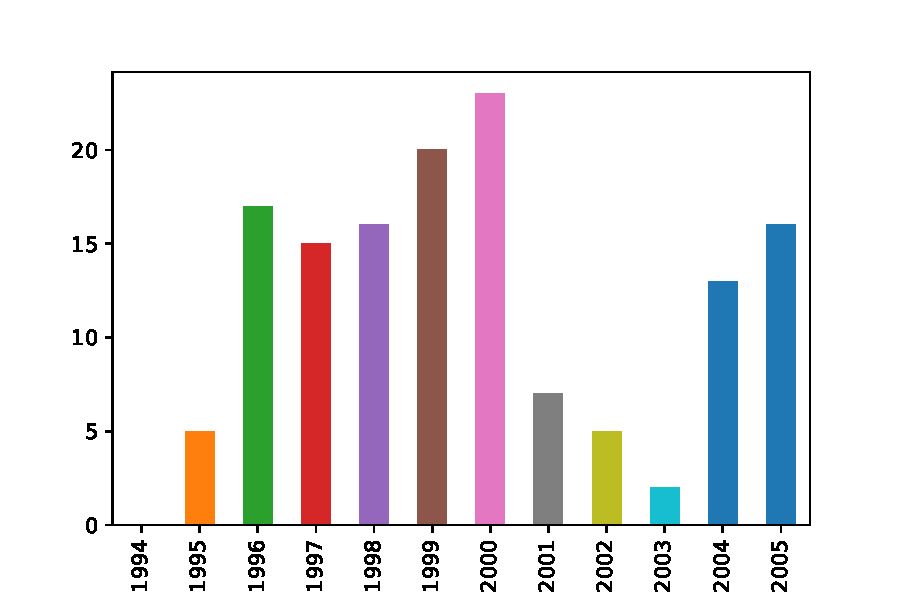
\includegraphics[page=1,width=.9\textwidth]{fig2.pdf} \\
   \end{tabular}
\end{figure}

%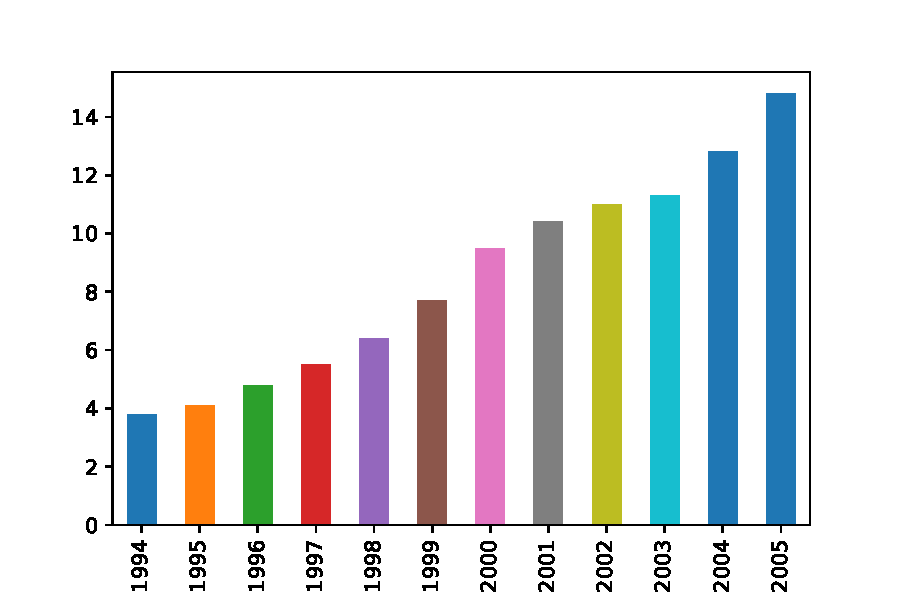
\includepdf{fig.pdf}
%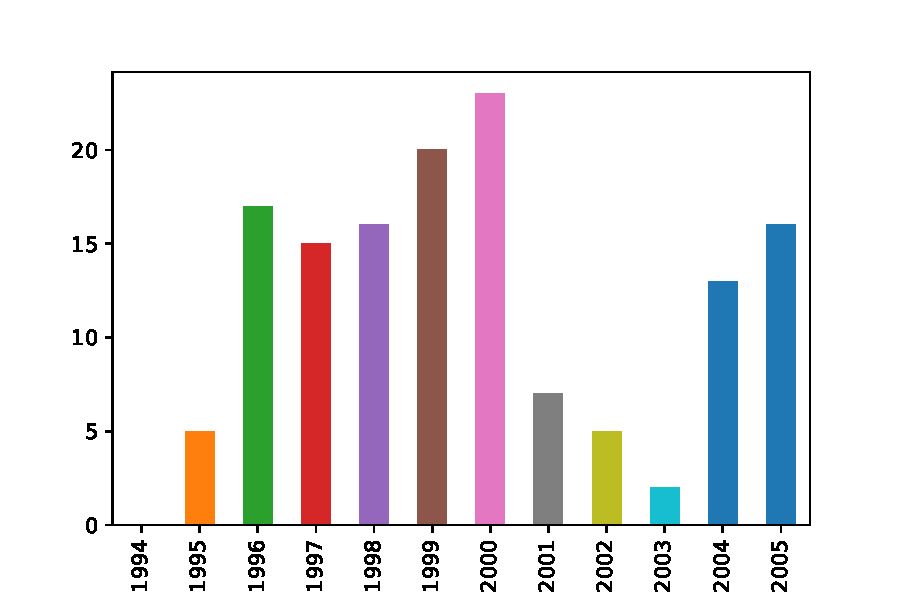
\includepdf{fig2.pdf}

\subsection{References}
\begin{thebibliography}{9}
    \bibitem{tittle2018control}
    Tittle, C. R. (2018). Control balance: Toward a general theory of deviance. Routledge.
    \bibitem{anderson2018policy}
    Anderson, E. (2018). Policy Entrepreneurs and the Origins of the Regulatory Welfare State: Child Labor Reform in Nineteenth-Century Europe. American Sociological Review, 83(1), 173-211.
    \bibitem{publichearing1998}
    United States. International Child Labor Program. (1998). Public hearings on international child labor. United States:Page:183
\end{thebibliography}
\end{document}